%!TEX root = ../dissertation.tex
\chapter{Industrial Use Case}
\label{industrial-use-case}

In this chapter will be presented a use case for the developed sentiment analysis model. For an initial test have been crawled new data focused on the target subject, and after been processed for the sentiment classification, have been presented with the Oracle Data Visualization Desktop tool. In the following paragraphs it will be discussed all the followed steps, and finally some information that have been extracted from the data.

\section{New Data Gathering}

For a preliminary use case of the sentiment analysis classification model discussed so far, it has been decided to introduce new information reputed useful for marketing analyses, with respect to the ones discussed for the yet gathered dataset. 



\section{Data Visualization}


\begin{figure}[ht]
	\centering
	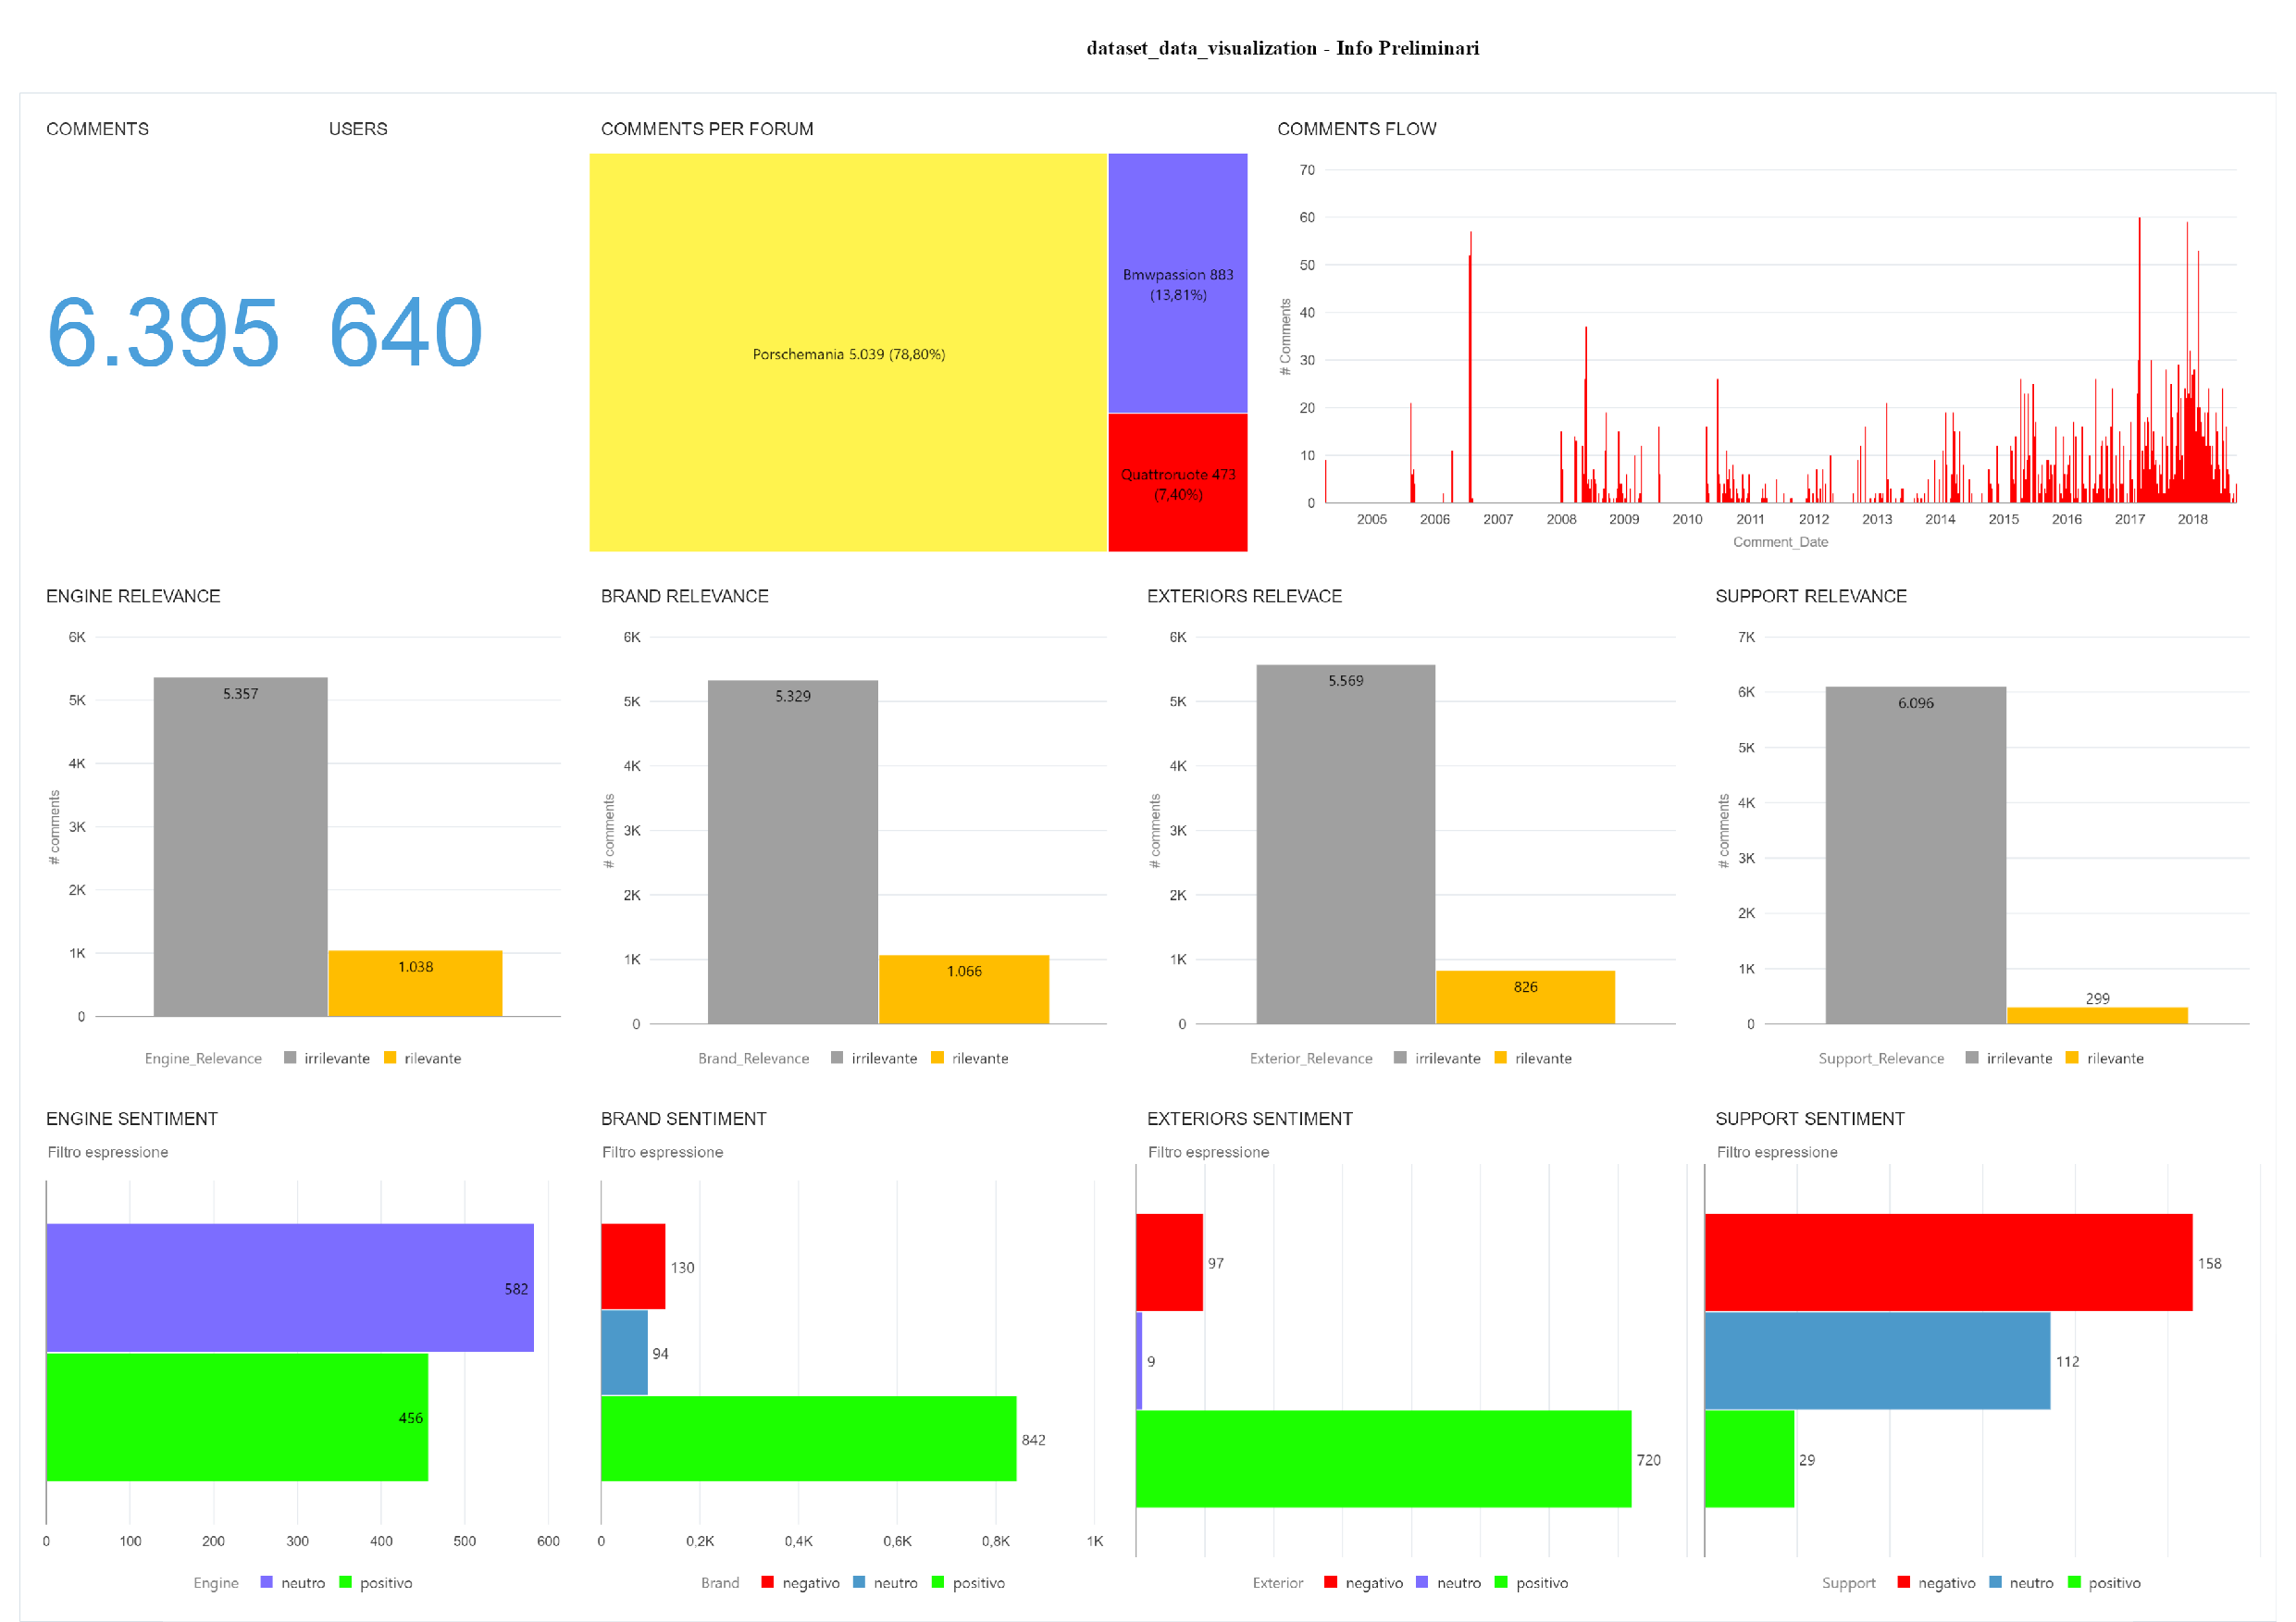
\includegraphics[width=\textwidth]{figures/odv_export/dataset_data_visualization_1.pdf}
	\caption{Overall statistics about the sentiment.}
	\label{fig:preliminar-info}
\end{figure}


\begin{figure}[ht]
	\centering
	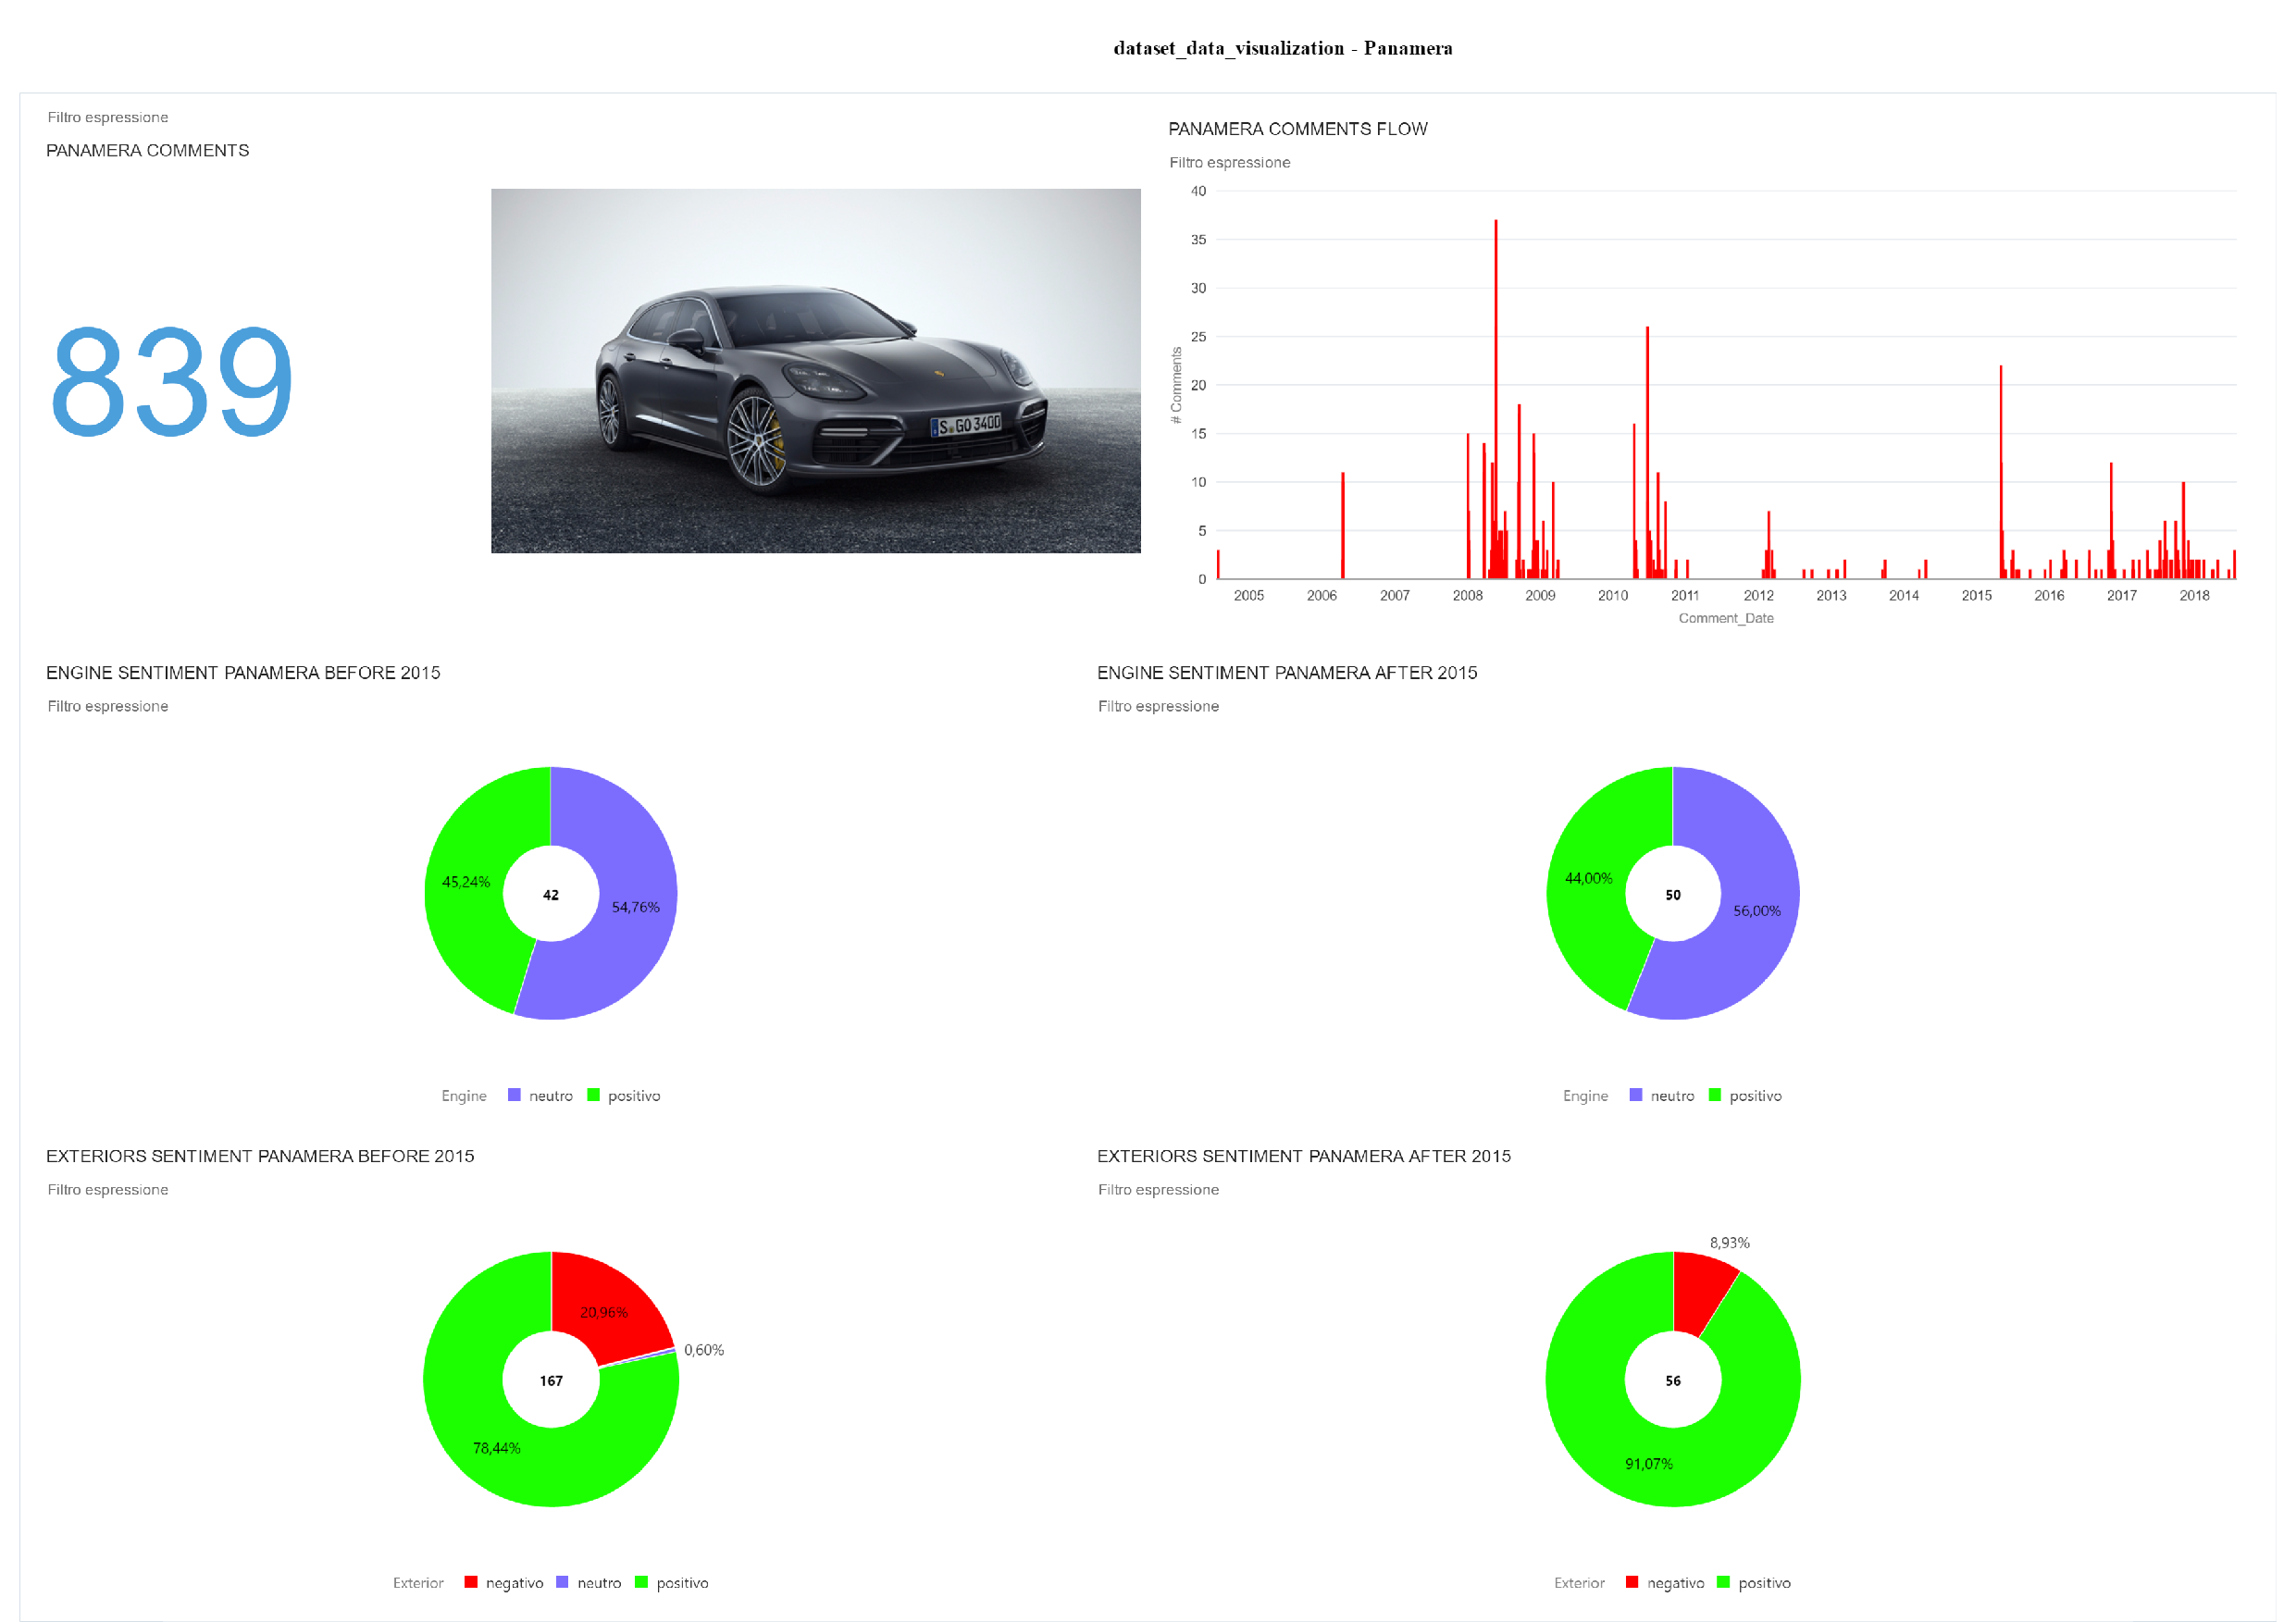
\includegraphics[width=\textwidth]{figures/odv_export/dataset_data_visualization_2.pdf}
	\caption{Sentiment polarities about Panamera model.}
	\label{fig:panamera-snt}
\end{figure}


\begin{figure}[ht]
	\centering
	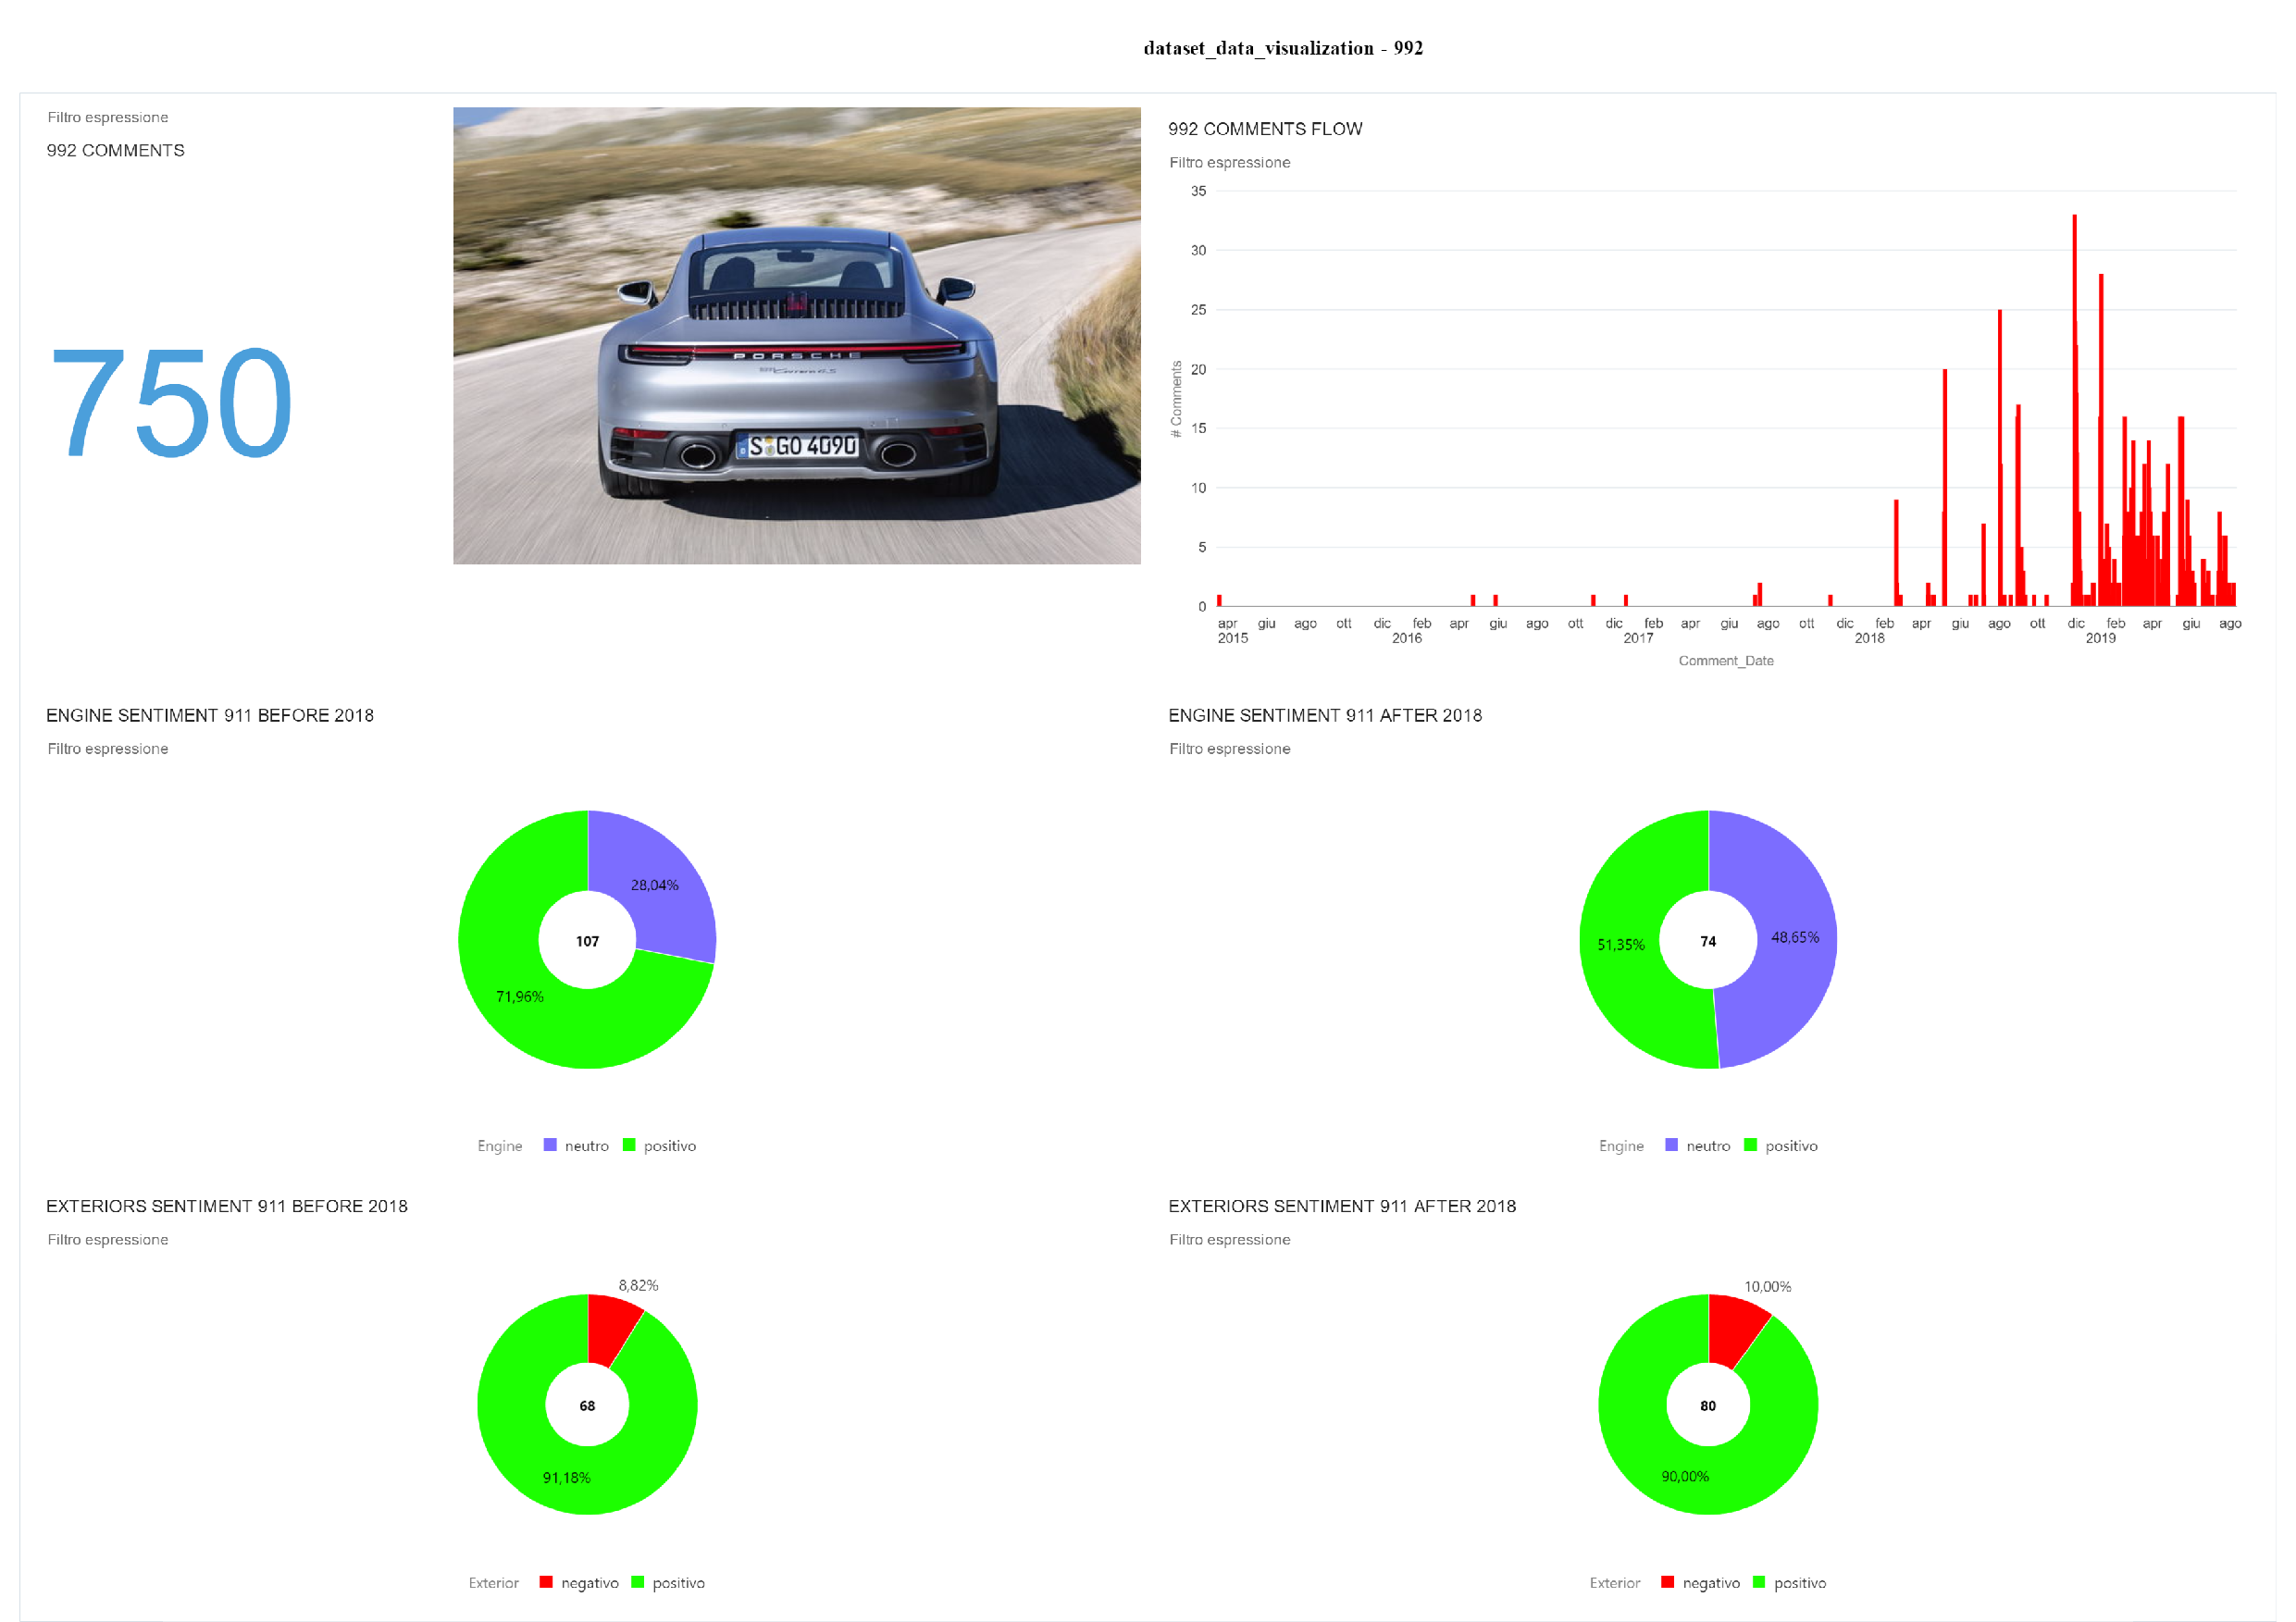
\includegraphics[width=\textwidth]{figures/odv_export/dataset_data_visualization_4.pdf}
	\caption{Sentiment polarities about 911 (992 version) model.}
	\label{fig:992-snt}
\end{figure}


\begin{figure}[ht]
	\centering
	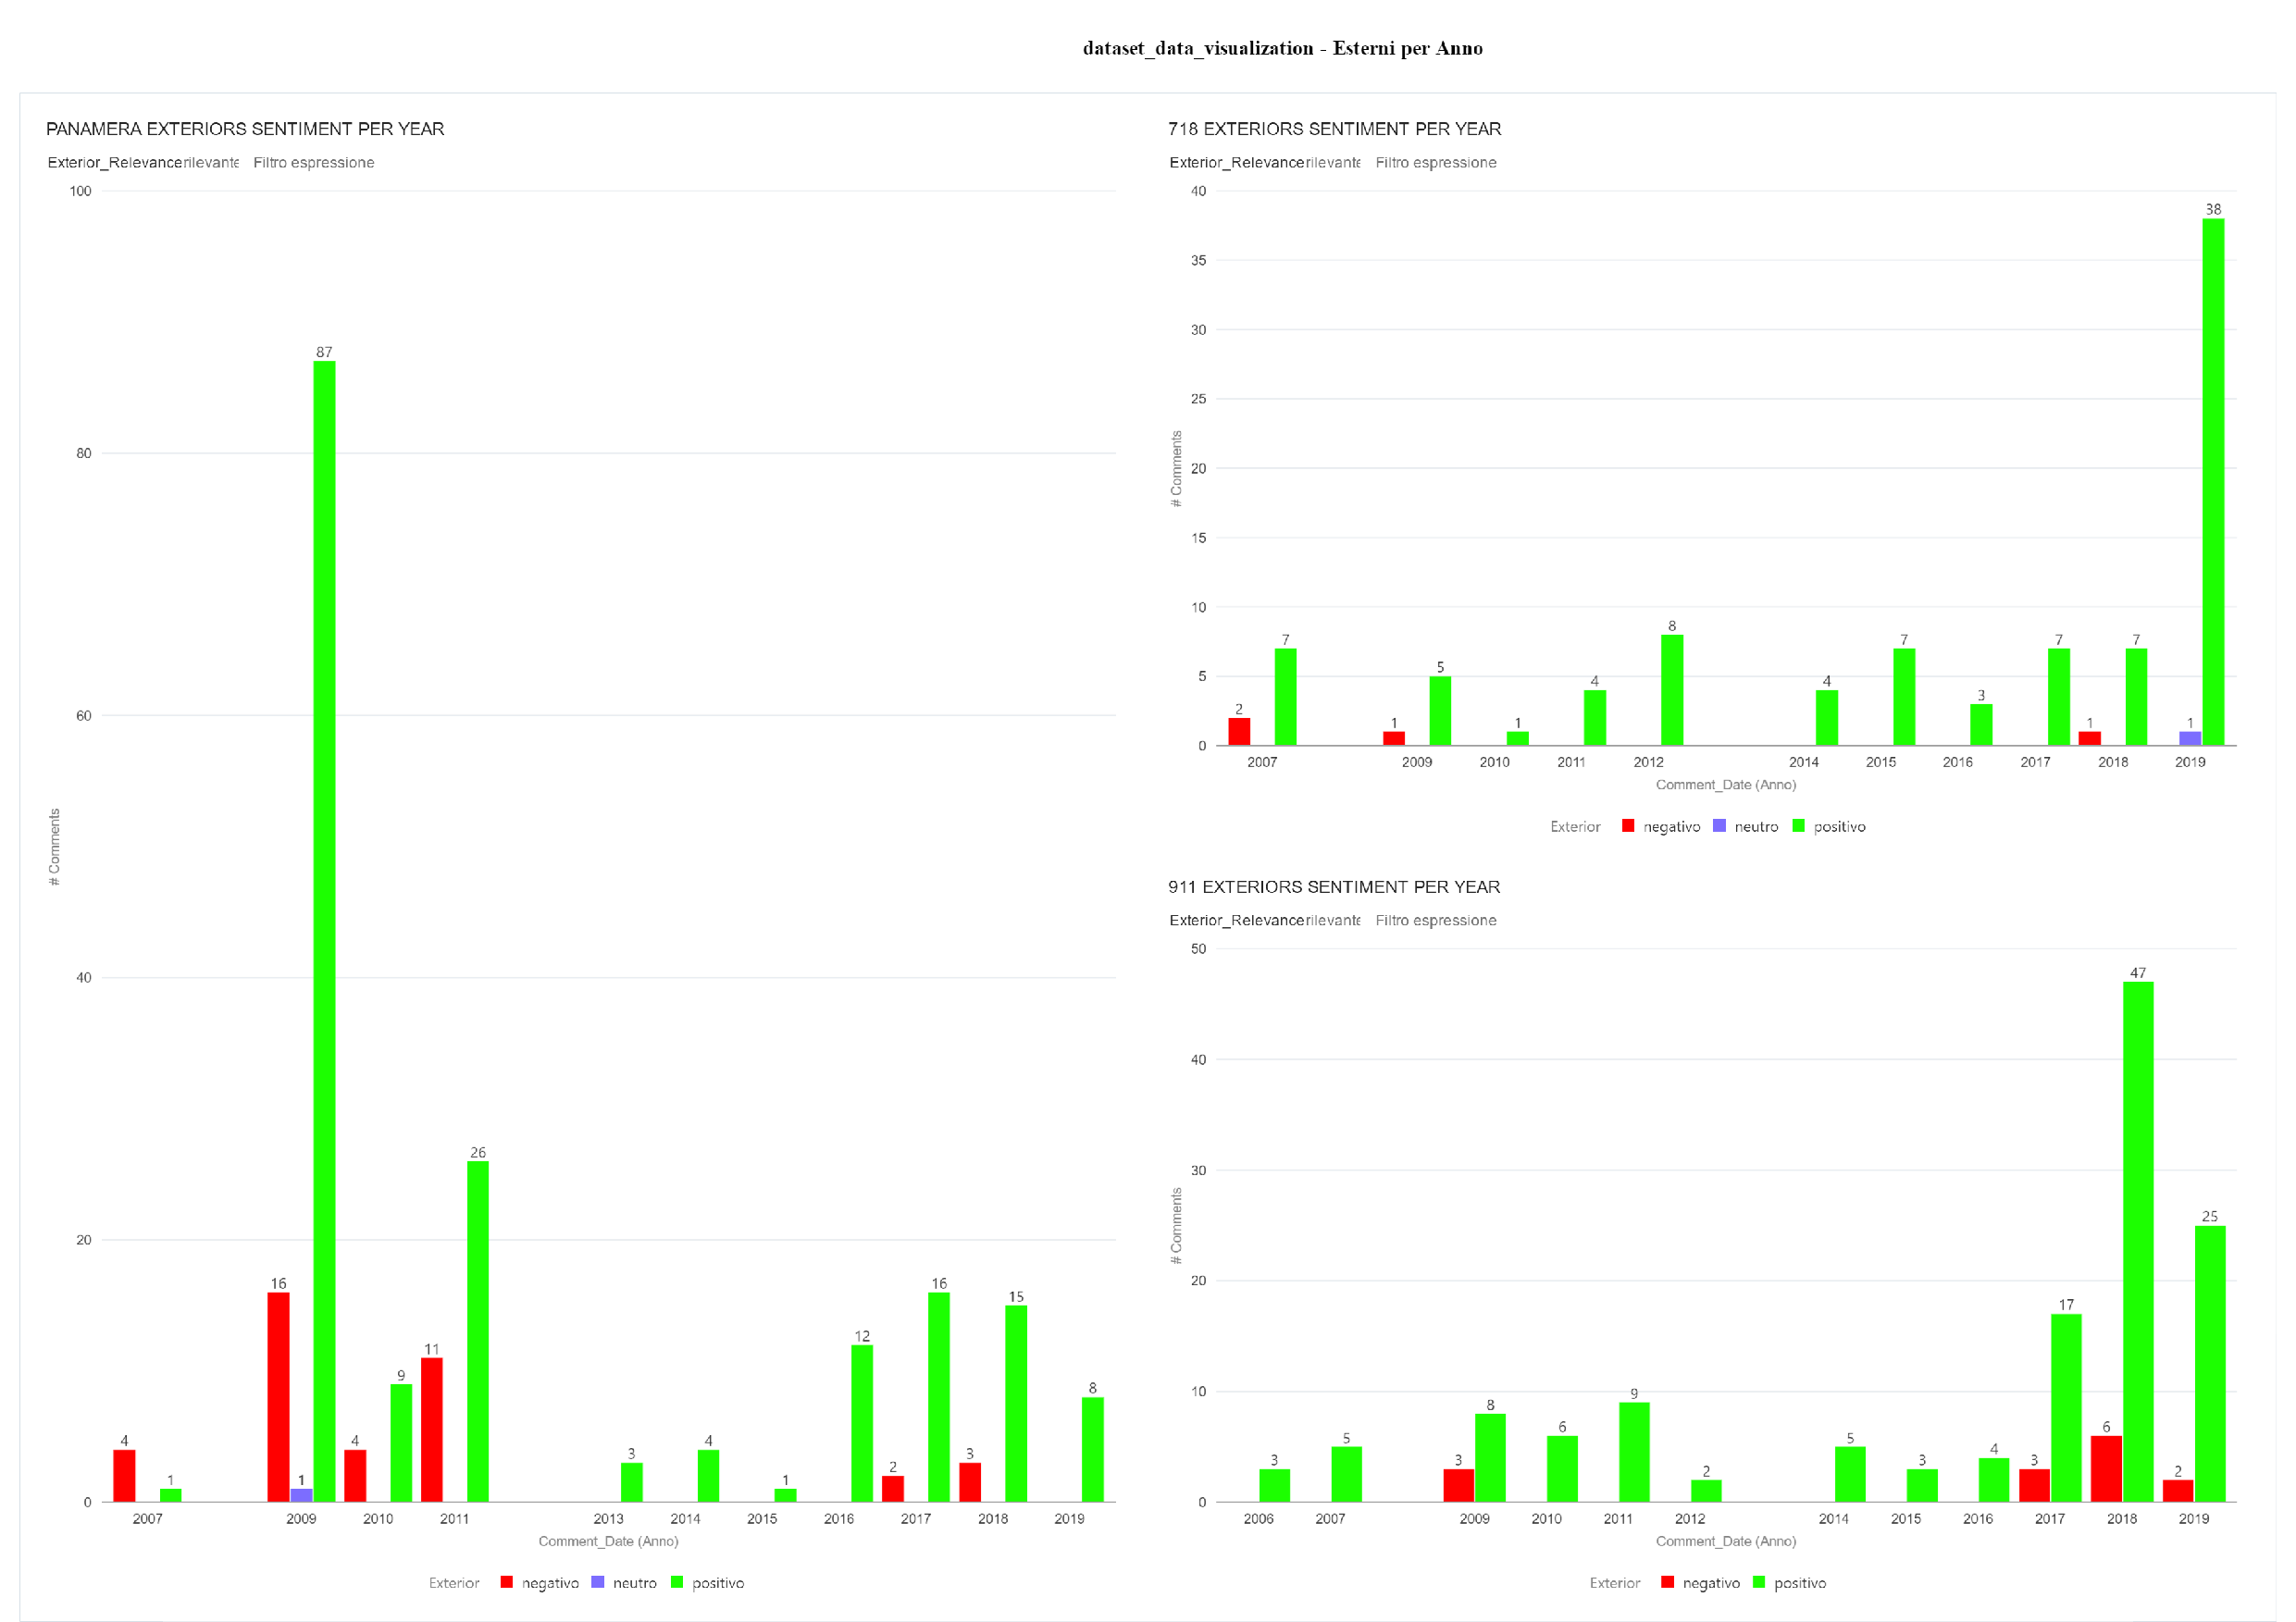
\includegraphics[width=\textwidth]{figures/odv_export/dataset_data_visualization_5.pdf}
	\caption{Sentiment polarities of some models on the years.}
	\label{fig:ext-year-snt}
\end{figure}


\begin{figure}[ht]
	\centering
	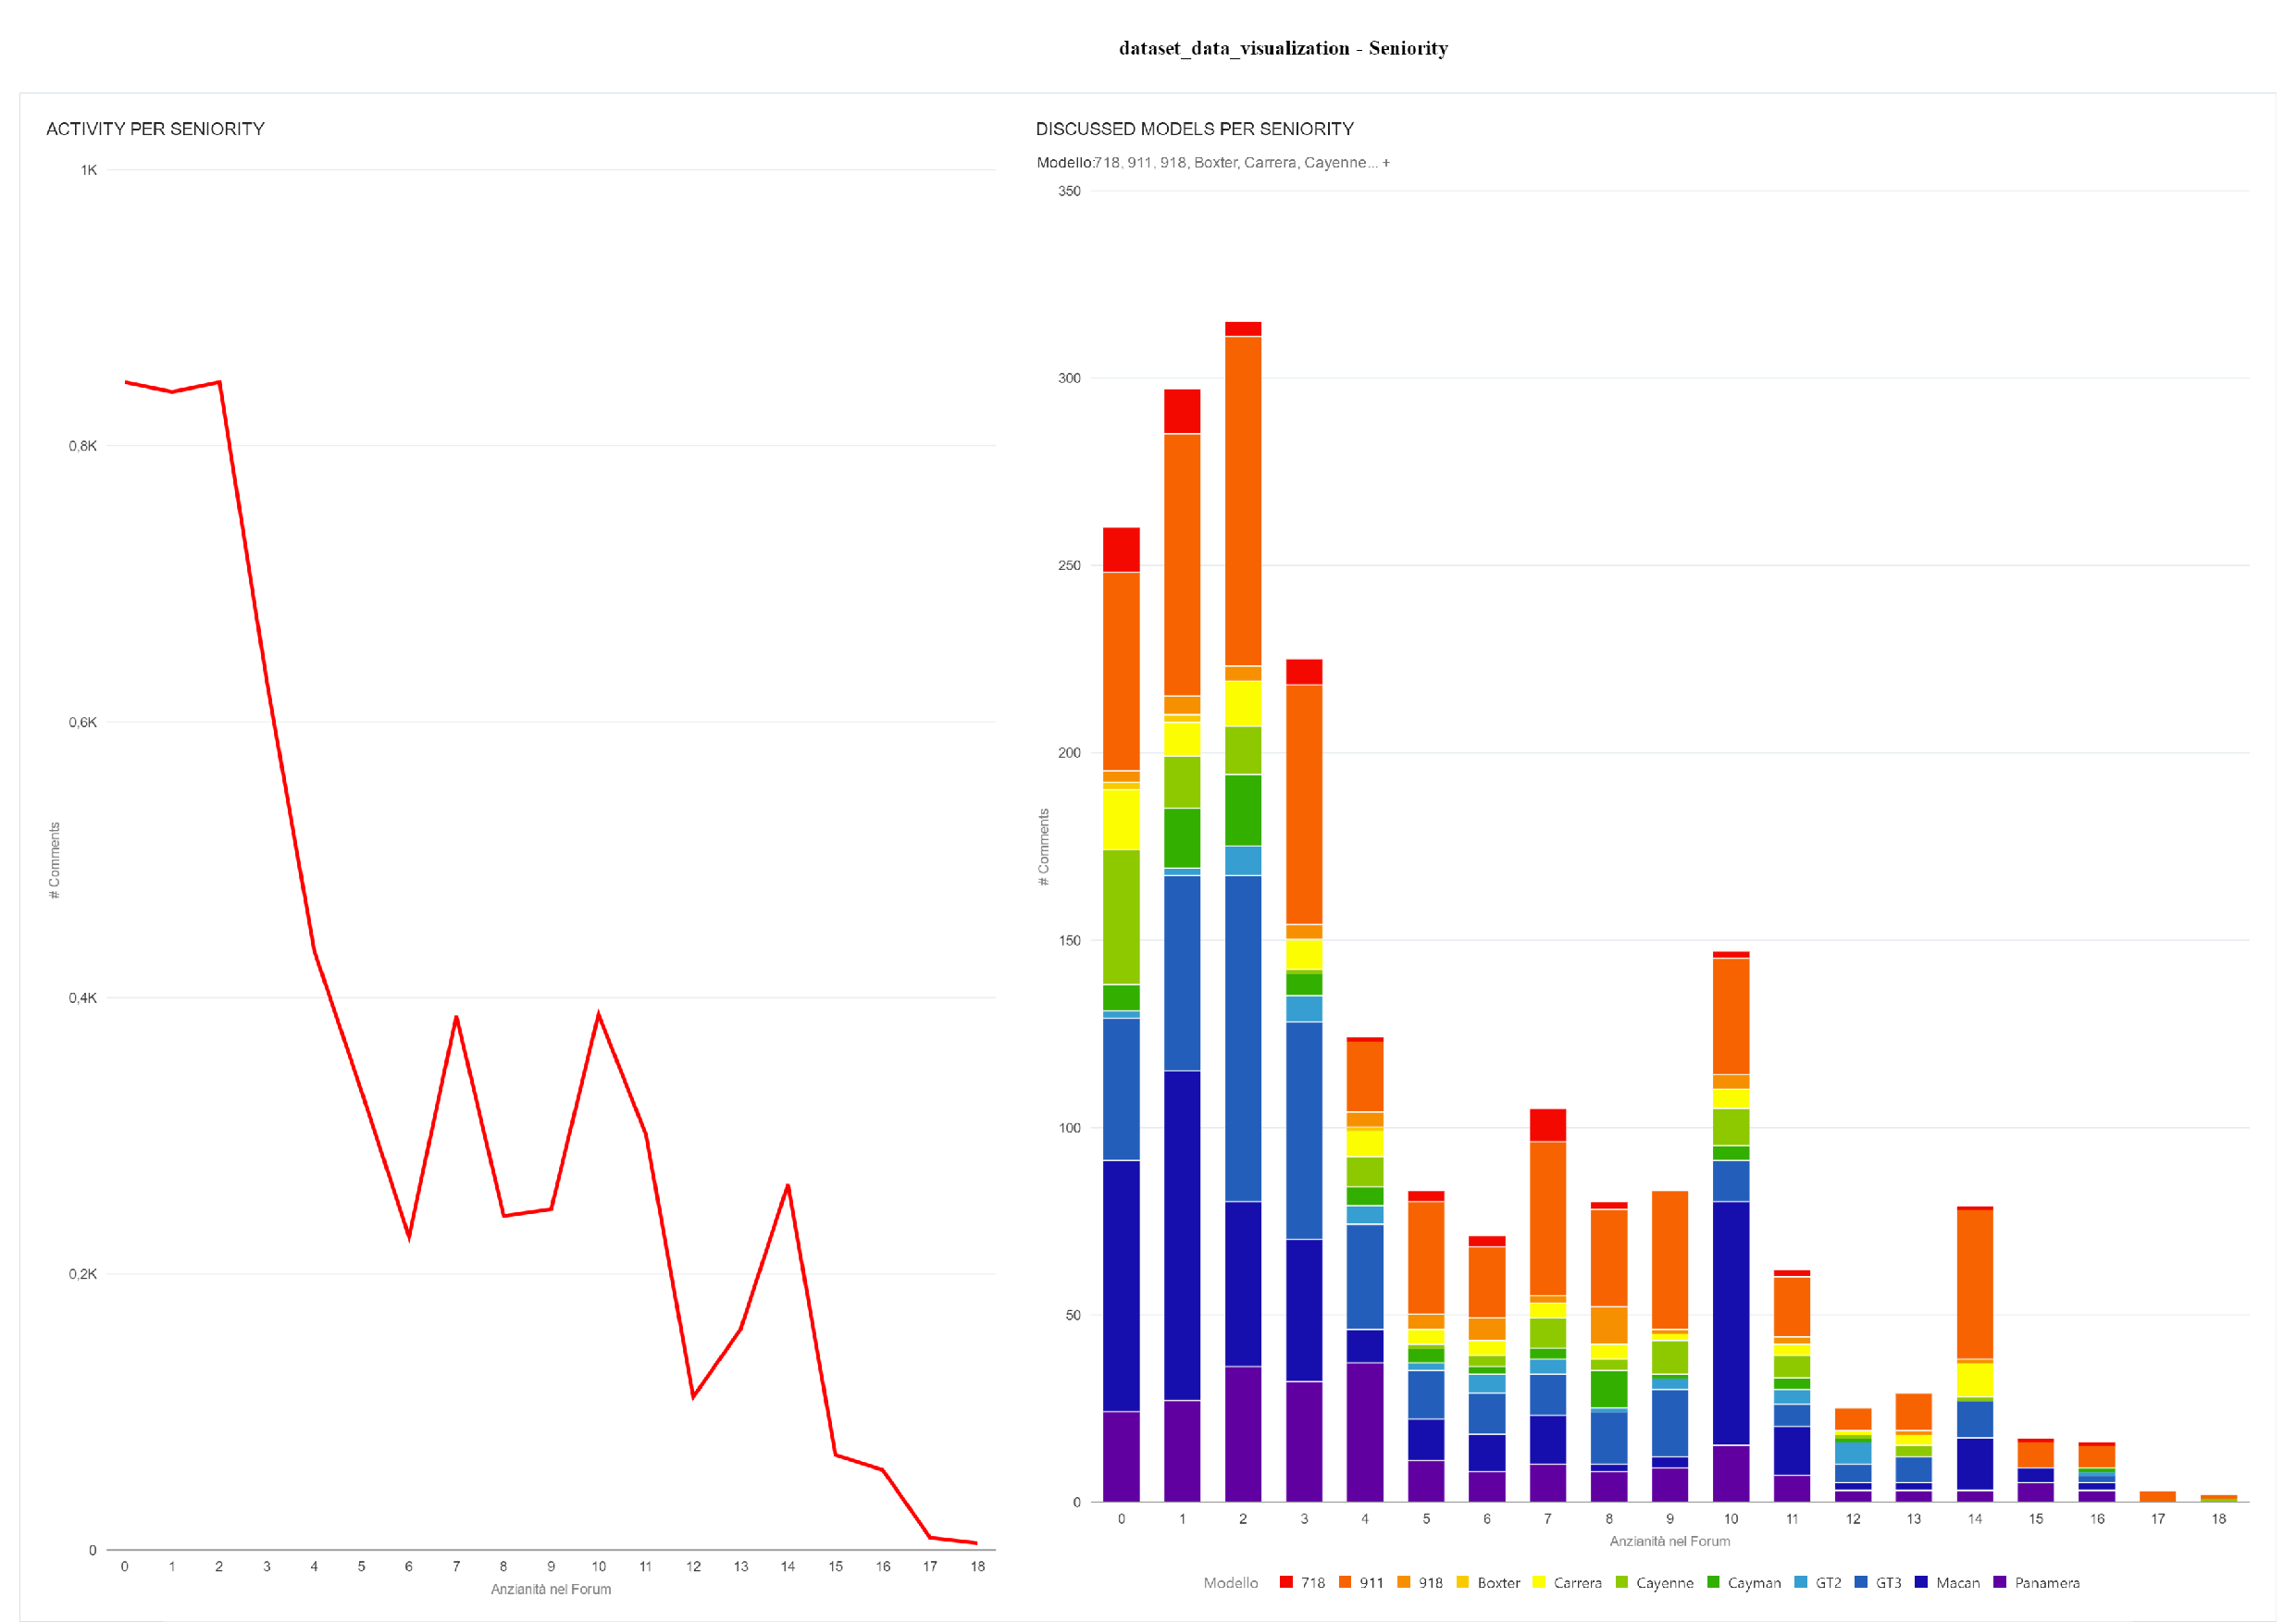
\includegraphics[width=\textwidth]{figures/odv_export/dataset_data_visualization_9.pdf}
	\caption{Models discussed per users' seniority.}
	\label{fig:model-senior}
\end{figure}


\begin{figure}[ht]
	\centering
	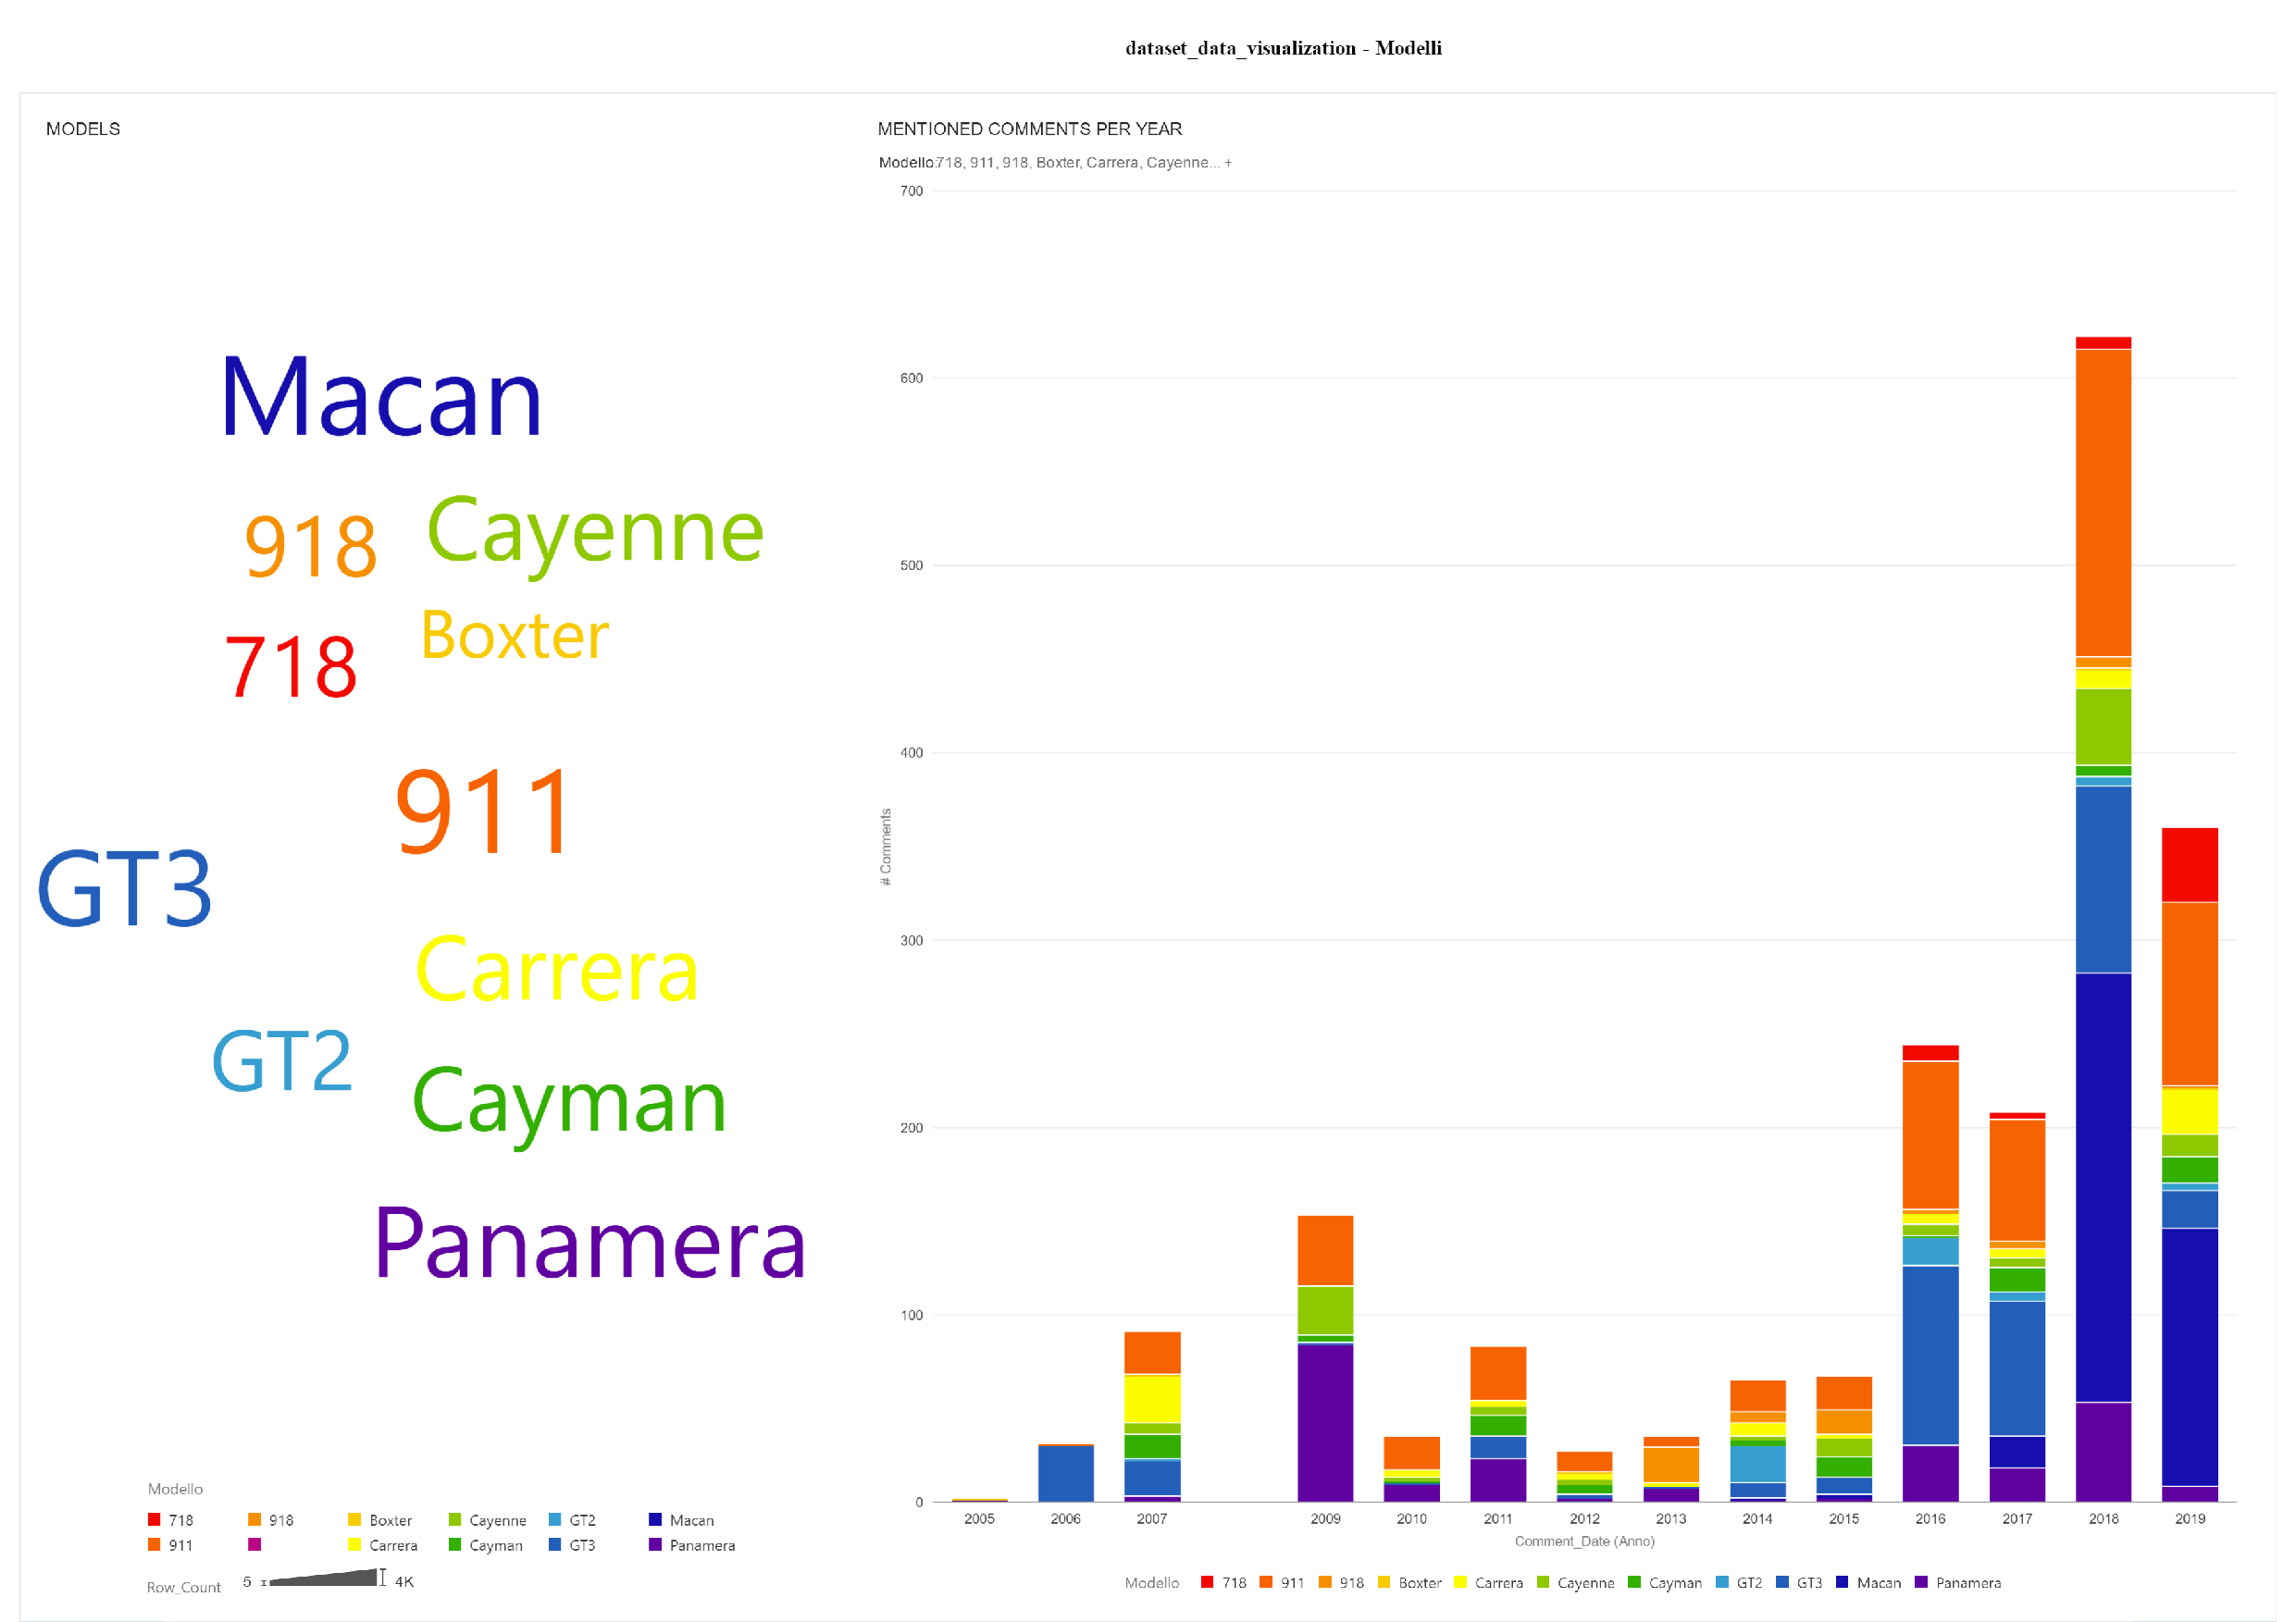
\includegraphics[width=\textwidth]{figures/odv_export/dataset_data_visualization_13.pdf}
	\caption{Most discussed models.}
	\label{fig:models}
\end{figure}